% 3_methodology.tex

\cleardoublepage
\chapter{Launch Vehicle Baseline Design}\label{chapter:methodology}


This chapter presents the baseline three stage small satellite launch system utilised in this thesis. The launch system is launched vertically under rocket power, from a traditional small rocket launch facility. The SPARTAN vehicle is mounted to the front of the first stage rocket. This configuration allows the SPARTAN to take the brunt of the aerodynamic forces and heating, as well as allowing the use of the control surfaces of the SPARTAN. The SPARTAN is accelerated by the first stage rocket, to its minimum operating velocity, at which point separation occurs. The SPARTAN's four scramjet engines are ignited, and SPARTAN accelerated through the atmosphere, reaching approximately Mach 9. At this point, the specific impulse of the scramjet engines, and thus the efficiency of the SPARTAN, have decreased, and the third stage rocket is separated. The third stage rocket accelerates for a time, before cutting its engine and coasting out of the atmosphere. Once the rocket is exoatmospheric, the engine is reignited multiple times, performing first a circularisation burn, and then a Hohmann transfer to the intended orbit. Meanwhile, the SPARTAN banks and executes a fly-back manoeuvre to return to its initial launch site. The SPARTAN extends landing gear, and lands on a traditional runway in the style of a conventional aircraft. The SPARTAN is able to be rapidly refurbished and remounted for further launches. 


\begin{figure}
	\centering
	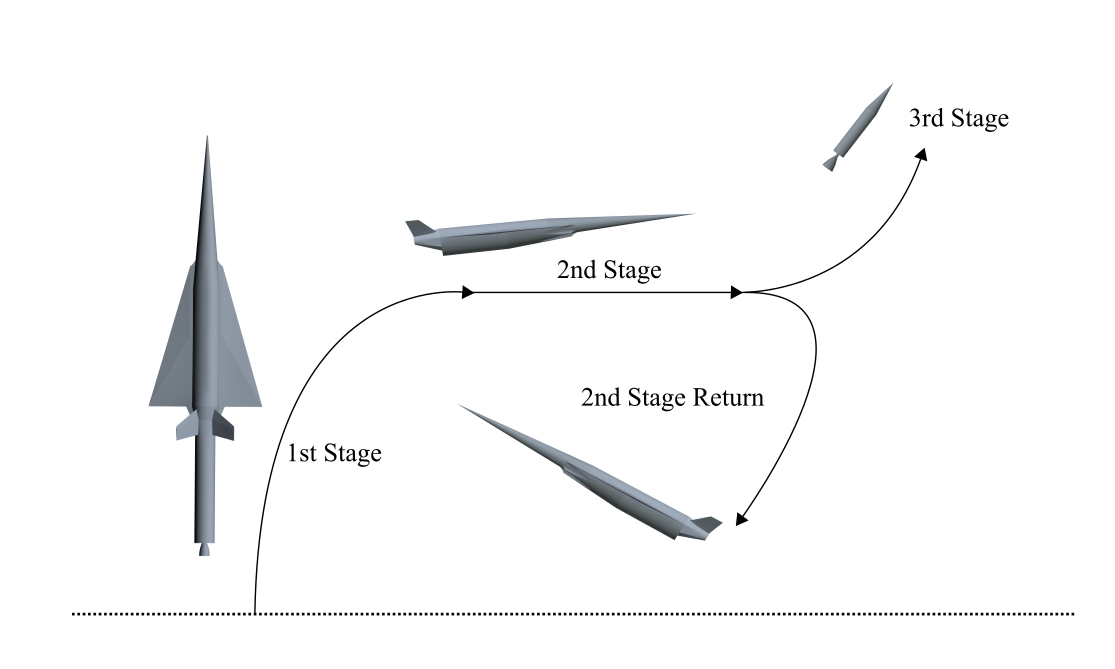
\includegraphics[width=0.9\linewidth]{figures/3_vehicle_design/Trajsimple}
	\caption{The launch process of the rocket-scramjet-rocket launch system, presented in simplified form.}
	\label{fig:Trajsimple}
\end{figure}

The design for the first stage rocket-powered vehicle, second stage scramjet-powered vehicle (the SPARTAN), and third stage rocket-powered vehicle are presented. This baseline design is used for the initial trajectory analysis and optimisation in this study. The launch system has been designed based on the SPARTAN vehicle developed by Preller \& Smart. The size and external design of the SPARTAN are used exactly as defined by Preller \& Smart, and are not modified in any way. The internal component masses of the SPARTAN are either identical to those defined by Preller \& Smart, or are scaled if the internal component is modified. The first stage rocket, third stage rocket, and internal components have been designed to conform to the size and shape of the baseline SPARTAN vehicle as defined by Preller \& Smart.

This chapter also describes the aerodynamic models of the vehicles used in this study, including the engine models.


\begin{figure}
\centering
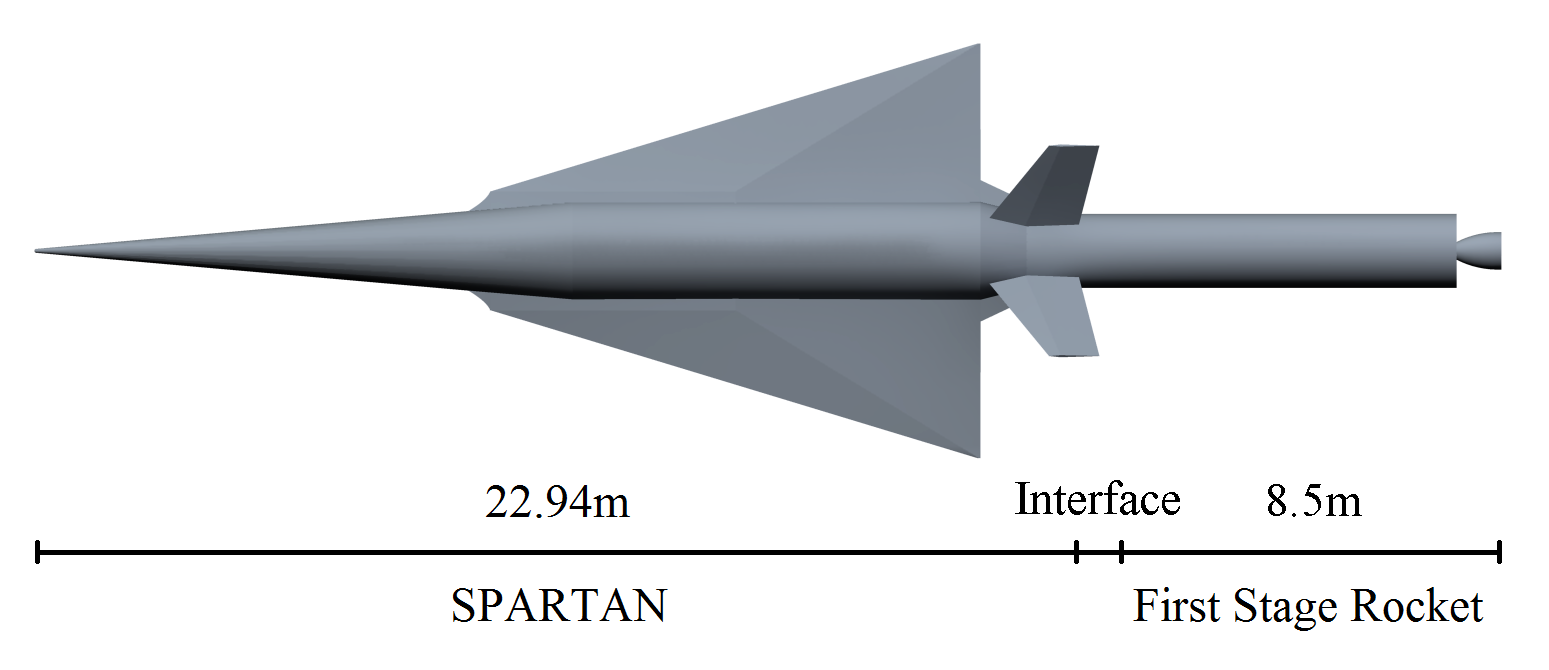
\includegraphics[width=0.7\linewidth]{figures/3_vehicle_design/NoInternal}
\caption{The rocket-scramjet-rocket launch system, top view, showing the SPARTAN and first stage.}
\label{fig:NoInternal}
\end{figure}

\begin{figure}
\centering
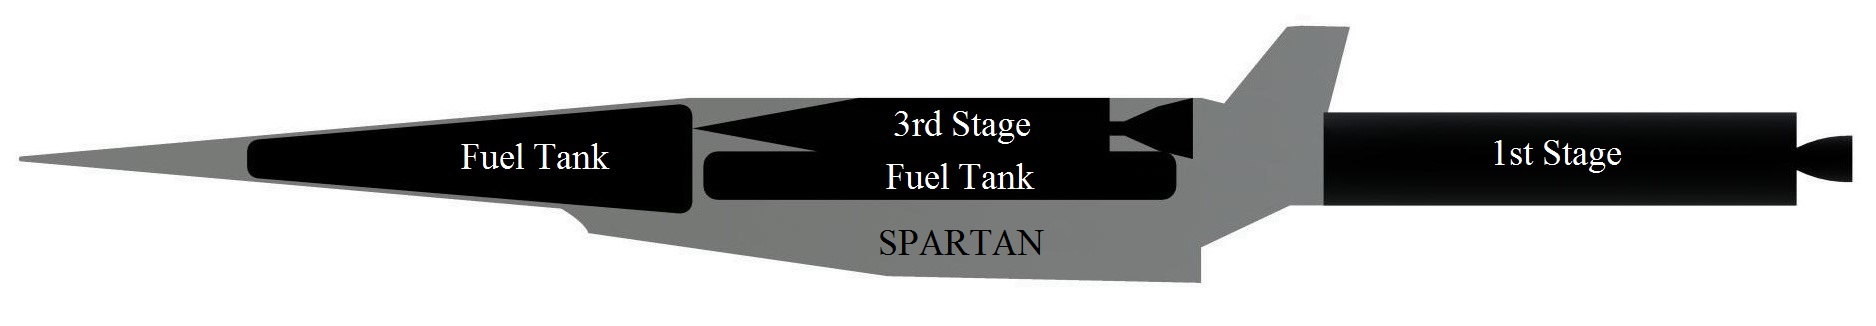
\includegraphics[width=0.7\linewidth]{figures/3_vehicle_design/INTERNALS}
\caption{The rocket-scramjet-rocket launch system, side view, showing the SPARTAN and fuel tanks, along with the third and first stages.}
\label{fig:INTERNALS}
\end{figure}



	
	
	\section{Second Stage Scramjet}
		\subsection{Baseline Vehicle}
		The SPARTAN vehicle in this study has been designed based on the work by Preller \& Smart CITATION. 
		
		The baseline SPARTAN has been designed to hold a 9 m long third stage.  Two cylindrical tanks underneath the third stage and a conical tank situated in the nose have a total volume of 22.0m3 and hold a total of 1562kg of LH2 fuel. This assumes an LH2 density of 71kg/m3, slightly denser than LH2 at phase transition point at 1 atm.
		
		 %http://webbook.nist.gov/cgi/fluid.cgi?Action=Load&ID=C1333740&Type=SatT&Digits=5&PLow=.5&PHigh=1.5&PInc=.1&RefState=DEF&TUnit=K&PUnit=atm&DUnit=kg/m3&HUnit=kJ/mol&WUnit=m/s&VisUnit=uPa*s&STUnit=N/m%
		
		
		The fuel tanks are sized to fit around the kestrel-powered third stage, described in Section XX. 
The fuel tanks have a total tank volume of 22.0m$^3$, containing a fuel mass of 1562kg.
The mass of the fuel tanks is scaled from Dawid Prellers model of the SPARTAN, giving a total fuel tank mass of 179.41kg.
		
		-detail individual fuel tank masses (and how they were designed)




\subsection{Propulsion Modelling}

\textcolor{red}{conical shock calcs}

\textcolor{red}{C-REST thrust calculator method?}

\textcolor{red}{be more quantitative, include control law for mass flow rate (eq=1?)}
The SPARTAN is powered by four underslung scramjet engines. These engines are Rectangular To Elliptical Shape Transition (REST) engines, configured to allow for a conical forebody (C-REST). The engine model used is a CRESTM10 database\cite{Preller2017}, analysed using quasi-1D simulation.
This database provides data points of engine performance over inlet conditions within the operational range, at 50kPa dynamic pressure equivalent conditions. The specific impulse and equivalence ratio data sets are shown in Figure XXX. This data is interpolated for the given inlet conditions to calculate the exit conditions and the specific impulse produced by the engine. The specific impulse is obtained by spline interpolation. The thrust, $T$, is then obtained by inclusion of the mass flow rate ($\dot{m}$) obtained via the inlet conditions, ie. $T = g_0\dot{m}I_{sp}$.
The C-REST engine is a fixed geometry engine, designed for operability at high Mach numbers\cite{Preller2017}. At lower Mach numbers, the addition of excessive fuel may cause the engine to choke and unstart, resulting in total loss of thrust\cite{Preller2017}. To avoid unstart, an equivalence ratio ($\phi$) of less than 1 is set at low Mach numbers. As the equivalence ratio is equal to 1 in the majority of the Mach number and temperature regime, only the regions in which it is less than 1 are used for the interpolation. The equivalence ratio interpolation is linear, as the number of data points available for interpolation is low. 

During flight the C-REST inlet conditions will stay within the region bounded by the available data. However, for the purposes of the pseudospectral method solver, it is necessary for the vehicle model to be able to extrapolate for ISP and equivalence ratio data. 

\begin{figure}
	\centering
	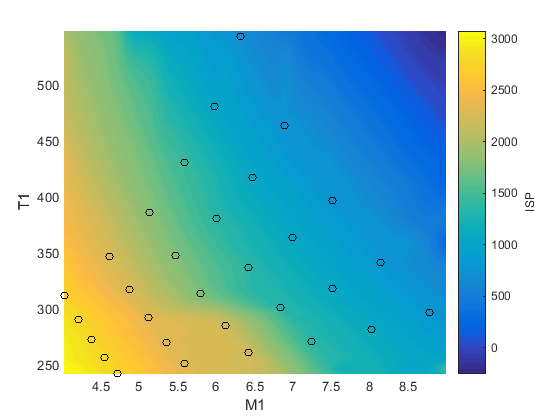
\includegraphics[width=0.7\linewidth]{figures/3_vehicle_design/ISPinterp}
	\caption{}
	\label{fig:ISPinterp}
\end{figure}
\textcolor{red}{Put Plot of eq Here too}


		
		
		\subsection{Aerodynamics}
		An initial surface triangulation of the SPARTAN has been created in Pointwise, shown in Figure \ref{fig:Pointwise}.
		\begin{figure}
			\centering
			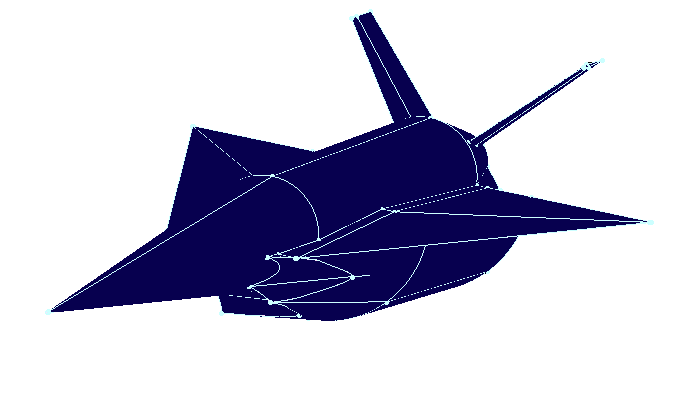
\includegraphics[width=0.7\linewidth]{figures/3_vehicle_design/Pointwise}
			\caption{}
			\label{fig:Pointwise}
		\end{figure}
		
		The aerodynamics of the SPARTAN have been calculated using CART3D, an inviscid CFD package used in the preliminary design of aerospace vehicles. Cart3D utilises adjoint mesh adaption with a Cartesian cut-cells approach to produce an iteratively refined mesh to fit a flow solution. CART3D has
		been used to generate the aerodynamic database of the SPARTAN vehicle due to its applicability in both the subsonic
		and supersonic regimes, and its robustness across multiple flow solutions [16]. CART3D has previously been used to
		analyse hypersonic vehicles, and has shown fair agreement with experimental data across multiple studies CITATIONXX.
		
		The SPARTAN encounters a large range of flight conditions during its launch and return flights. During launch, and some sections of the return flight, the scramjet engines are turned on. While during the majority of the return flight, the scramjet engines are not operational, and air flows through the flowpath without fuel injection. The engines change the aerodynamics of the SPARTAN considerably. When the engines are not powered on, the flowpath generates a large amount of drag. When the engines are powered on, the engines are generating thrust on the internal nozzle, as well as on the boat-tail and base. The engine-on aerodynamics are described in Section \ref{sec:engine-on}.
		
		The aerodynamics of the SPARTAN are calculated using for Mach numbers from 0.2 to 10, and angle of attack values from 0$^\circ$ to 10$^\circ$. Engine-on aerodynamic calculations are performed for Mach numbers 5,7,9 and 10, and at altitudes from 20km to 40km. 
		
		details of CART3D setup (no adapt levels / radius etc)
		
		CART3D Meshes were initiated with an outer boundary distance of 40 times the vehicle length. This boundary distance was observed to produce suitable free stream conditions and good mesh convergence. Nine mesh adaption levels were used. Nine levels were observed to generally produce good convergence, with moderate computation times of 1-3 hours per simulation. The convergence of the residuals and forces were investigated to ascertain if a solution has converged. 
		
		
		CART3D validation
		
		
		Example cases are shown in Figure \ref{fig:M1}, \ref{fig:M3AoA6} and \ref{fig:M7AoA6}. Figures XXX and XXX show the lift and drag coefficients of the SPARTAN vehicle over the range of Mach numbers and angle of attack values analysed.
		
		
		
		
		method of calculating aerodynamics for trim at required lift
		
		-detail hypaero vs CART3D? 
		
		
		conical shock calculation
		
		
		
An initial centre of gravity of 14.0m was calculated using CREO, using the mass fractions calculated by Preller [CITATION]. This centre of gravity calculation assumes that the structural mass of the SPARTAN is evenly distributed throughout the body volume. As the SPARTAN is still in the preliminary design stages, it has been assumed that the centre of gravity is slightly variable. This assumption allows the centre of gravity to be varied slightly to improve the stability of the SPARTAN, as well as positioning the moment centre to minimise necessary flap deflection over the trajectory of the SPARTAN, improving the aerodynamic characteristics of the SPARTAN. 



The centre of gravity of the SPARTAN is varied as fuel is depleted throughout the acceleration phase, as well as when the third stage rocket is released. A point mass model is used in conjunction with the aerodynamic database,
and atmospheric properties obtained from the U.S Standard Atmosphere 1976[26]. The SPARTAN is assumed to be
trimmed at all conditions during flight.






  \subsubsection{Aerodynamics of SPARTAN Alone}
  
This section details the aerodynamics of the SPARTAN, calculated using CART3D. A SPARTAN model was provided for this study by Mr. Joseph Chai. A surface grid was created on this model using Pointwise\cite{Pointwise}. This model includes engine flowpaths. 






14.5m set as CG at end of burn, after third stage release. This is observed to produce a relatively stable trimmed acceleration and return. 

A total of 9 aerodynamic matrices are created
-CG no third stage, no fuel (assumed fly-back fuel does not change CG)
-CG third stage, no fuel
-CG third stage, full fuel

for each of these

-engine off coeffs
-engine on coeffs
-Flap Deflection coeffs


\begin{figure}
\centering
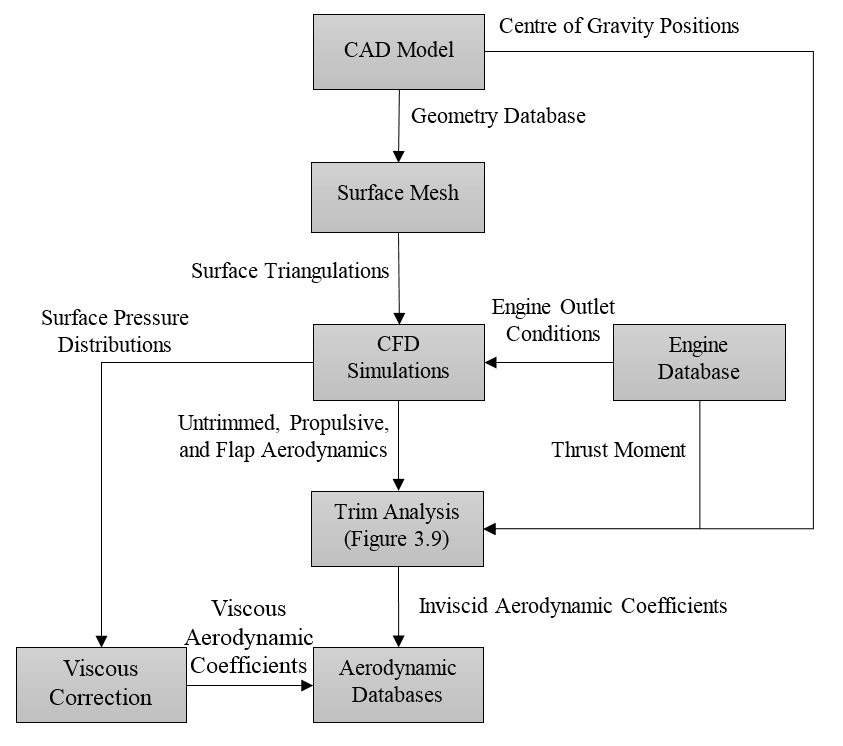
\includegraphics[width=0.7\linewidth]{figures/3_vehicle_design/FlowChart}
\caption{}
\label{fig:FlowChart}
\end{figure}


-show side and bottom results for M=0.5,1.1,5,9 (appendix)

\begin{figure}
	\centering
	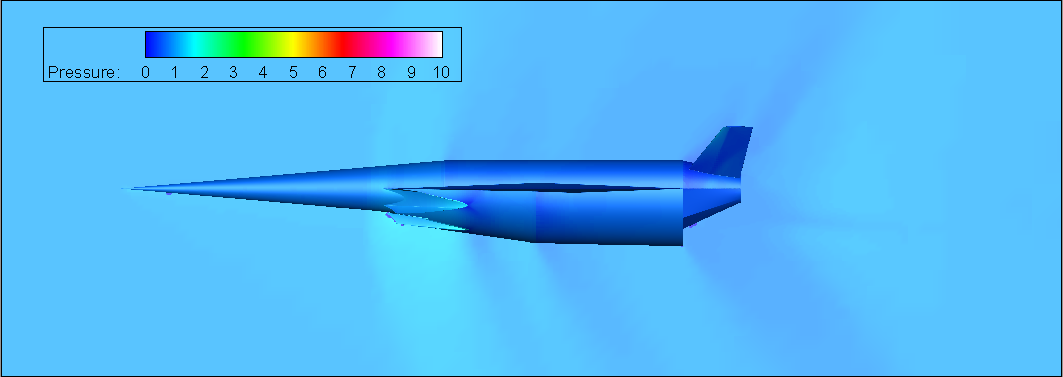
\includegraphics[width=0.9\linewidth]{figures/3_vehicle_design/M1p1AoA6}
	\caption{CART3D flow result for the SPARTAN, at Mach 1.1, 6$^\circ$ angle of attack.}
	\label{fig:M1}
\end{figure}
\begin{figure}
	\centering
	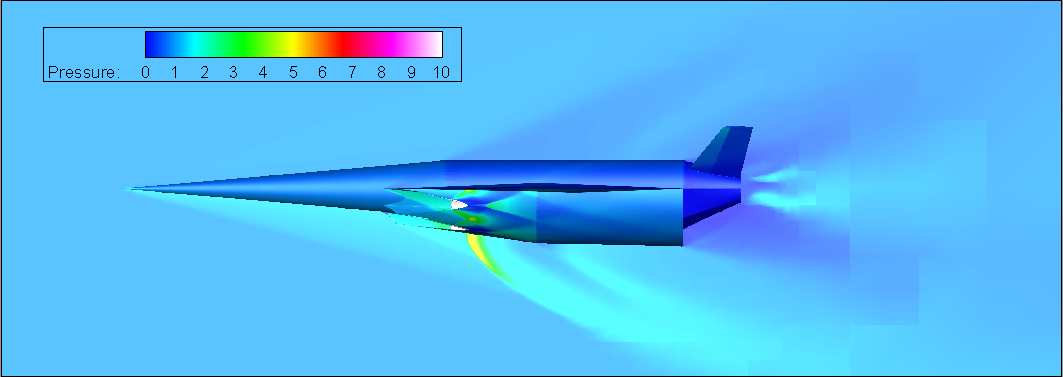
\includegraphics[width=0.9\linewidth]{figures/3_vehicle_design/M3AoA6}
	\caption{CART3D flow result for the SPARTAN, at Mach 3, 6$^\circ$ angle of attack.}
	\label{fig:M3AoA6}
\end{figure}
\begin{figure}
	\centering
	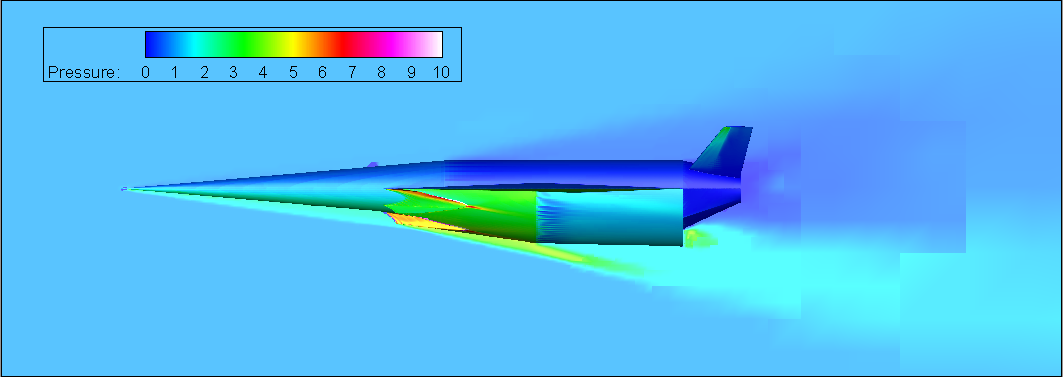
\includegraphics[width=0.9\linewidth]{figures/3_vehicle_design/M7AoA6}
	\caption{CART3D flow result for the SPARTAN, at Mach 7, 6$^\circ$ angle of attack.}
	\label{fig:M7AoA6}
\end{figure}


\textcolor{red}{need engine off, engine on and flap deflection comparisons}
CHANGE THESE GRAPHICS

\begin{figure}
	\begin{subfigure}{.5\textwidth}
\centering
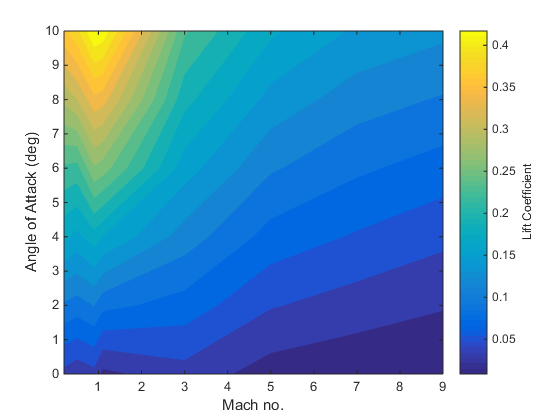
\includegraphics[width=0.99\linewidth]{figures/3_vehicle_design/Cl}
\caption{Coefficients of lift of the SPARTAN, calculated using CART3D.}
\label{fig:Cl}
\end{subfigure}
\begin{subfigure}{.5\textwidth}
\centering
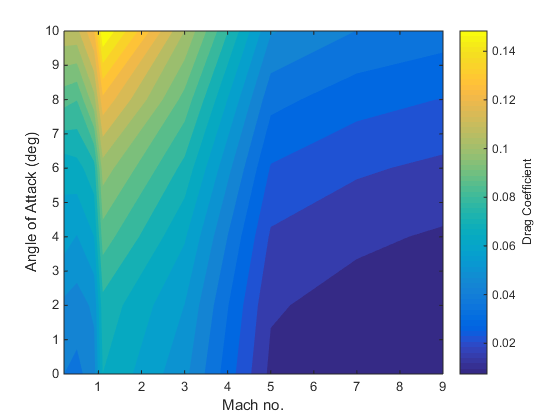
\includegraphics[width=0.99\linewidth]{figures/3_vehicle_design/Cd}
\caption{Coefficients of drag of the SPARTAN, calculated using CART3D.}
\label{fig:Cd}
\end{subfigure}
\begin{subfigure}{.5\textwidth}
\centering
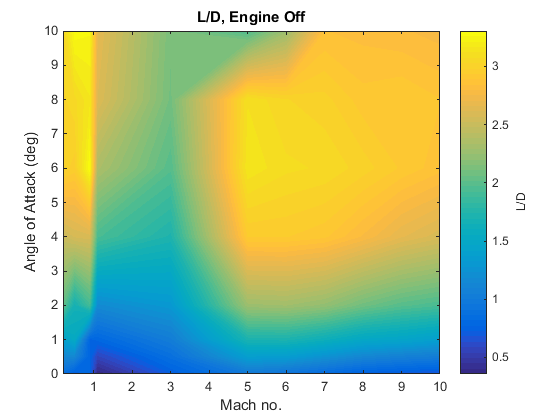
\includegraphics[width=0.99\linewidth]{figures/3_vehicle_design/LD}
\caption{L/D of the SPARTAN.}
\label{fig:LD}
\end{subfigure}
\end{figure}


These results show a distinct maximum region in the L/D of the SPARTAN at high Mach numbers, within the hypersonic regime. Below Mach 5, the L/D of the SPARTAN decreases sharply. 

\begin{figure}
	\begin{subfigure}{.5\textwidth}
	\centering
	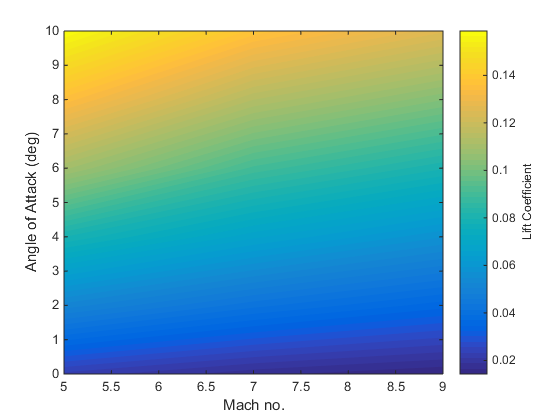
\includegraphics[width=0.99\linewidth]{figures/3_vehicle_design/Cl-EngineOn}
	\caption{Coefficient of lift of the SPARTAN with the C-REST engines powered-on. This is obtained by removing the engines and boat-tail from the CART3D simulation results.}
	\label{fig:Cl-EngineOn}
\end{subfigure}
\begin{subfigure}{.5\textwidth}
	\centering
	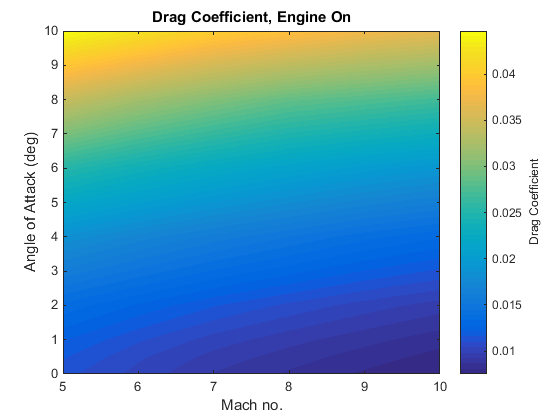
\includegraphics[width=0.99\linewidth]{figures/3_vehicle_design/Cd-EngineOn}
	\caption{Coefficient of drag of the SPARTAN with the C-REST engines powered-on. This is obtained by removing the engines and boat-tail from the CART3D simulation results.}
	\label{fig:Cd-EngineOn}
\end{subfigure}
\begin{subfigure}{.5\textwidth}
	\centering
	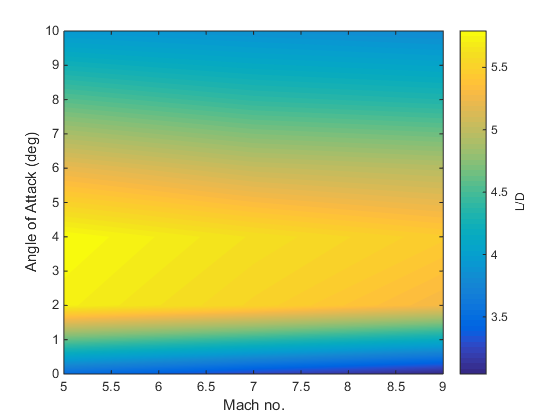
\includegraphics[width=0.99\linewidth]{figures/3_vehicle_design/LD-EngineOn}
	\caption{L/D of the SPARTAN with the C-REST engines powered on.}
	\label{fig:LD-EngineOn}
\end{subfigure}
\end{figure}

For the engine-on case, the engines and boat tail are removed from the aerodynamics of the vehicle. In the engine-on case the drag is decreased for all conditions. The lift is increased at low angle of attack, and increased at high angle of attack.




The SPARTAN is trimmed using control surfaces on the wings, shown in figure \ref{fig:SPARTAN_FLAPS}. 

\begin{figure}
	\centering
	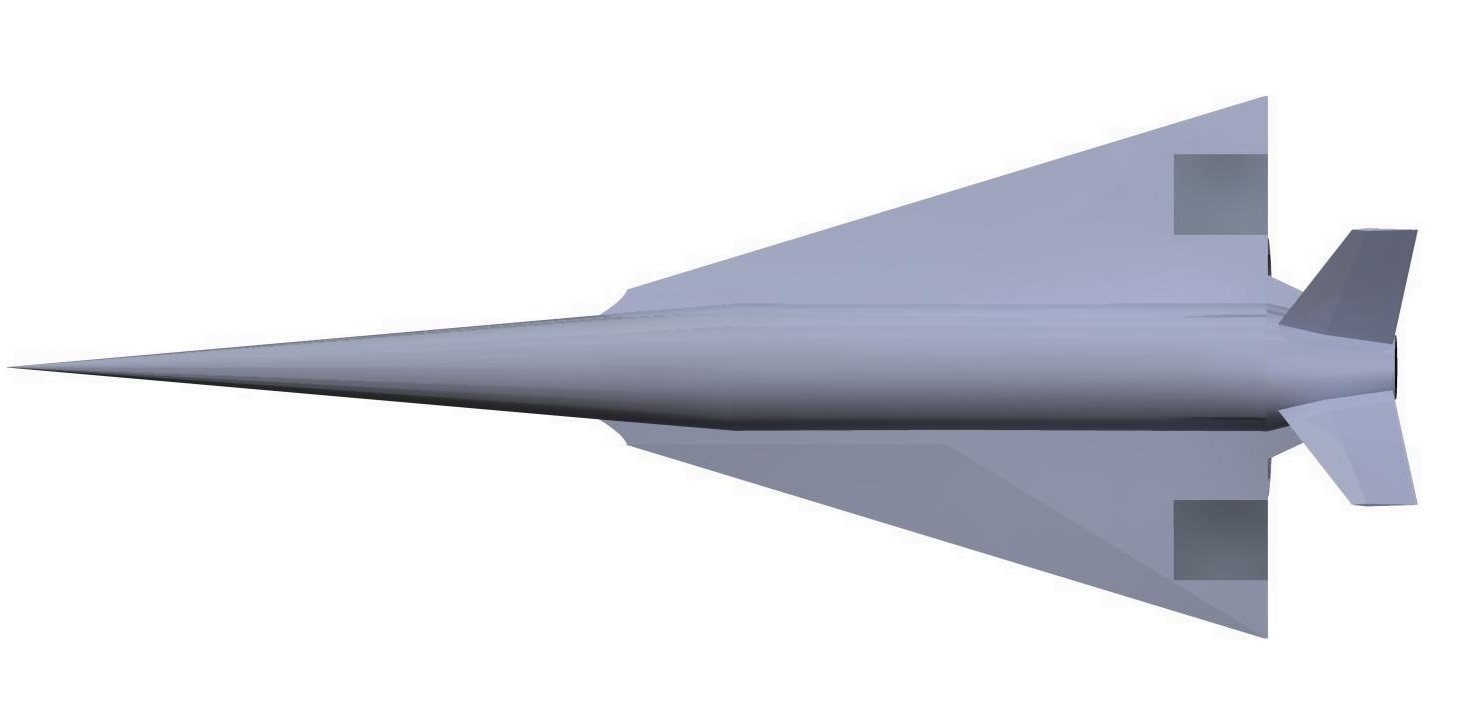
\includegraphics[width=0.7\linewidth]{figures/3_vehicle_design/SPARTAN_FLAPS}
	\caption{}
	\label{fig:SPARTAN_FLAPS}
\end{figure}


The trimmed aerodynamics of the SPARTAN are determined by modelling the flaps at deflected states of -20$^\circ$, -10$^\circ$, 10$^\circ$, and 20$^\circ$. Each of these deflected states were modelled in CREO and a surface mesh was created in Pointwise. The aerodynamics at each flap deflection were calculated at 0$^\circ$ angle of attack for Mach numbers between 0.2 and 10. Trim is determined by calculating the aerodynamic moment coefficient with zero flap deflection, then calculating the flap deflection necessary to balance the aerodynamic moments to zero. This trim balancing is calculated prior to trajectory optimisation for computational efficiency. For each aerodynamic data point of Mach numbers between 0.2 and 10, and angle of attacks from 0$^\circ$ to 10$^\circ$, the necessary flap deflection are calculated, and the additional lift and drag produced by the flaps are added. The addition of trimmed aerodynamics is calculated for scramjet engines on, and engines off conditions. Due to centre of gravity variation, the trim analysis is calculated three times; at the beginning of SPARTAN acceleration; at the end of SPARTAN acceleration, when fuel has been depleted; and after the third stage has been released. The trimmed aerodynamic databases at the beginning and end of acceleration are interpolated between as the centre of gravity varies due to fuel depletion. After the third stage is released, the centre of gravity is kept constant, and a single trimmed aerodynamic database is used. 

Figure \ref{fig:FlapDeflection} shows the necessary flap deflections to trim the SPARTAN. An Engine-on case is shown at a centre of gravity of  14.91m corresponding to full-fuel with third stage, and an Engine-off case is shown for a centre of gravity of 14.5m, corresponding to a fuel-empty state after third stage release. Additional figures illustrating the variation in moment coefficients are shown in Appendix XX.
The flap deflections are designated as negative up. Negative flap deflection necessary for trim indicates that the centre of pressure is aft of the centre of gravity, and that the vehicle has positive static margin, and is generally likely to be stable. Figure \ref{fig:FlapDeflectionENgineOn} and XX indicate that the SPARTAN is stable for 


\begin{figure}
\begin{subfigure}{.5\textwidth}
\centering
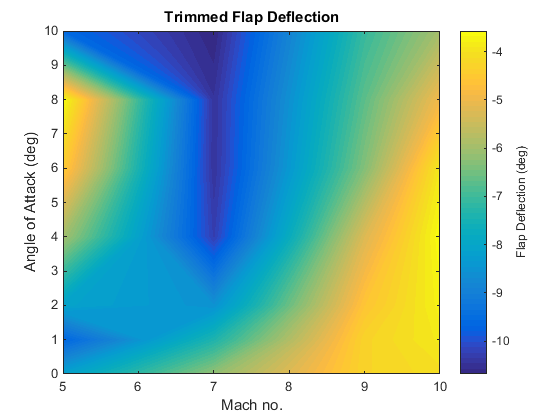
\includegraphics[width=0.99\linewidth]{figures/3_vehicle_design/FlapDeflectionENgineOn}
\caption{}
\label{fig:FlapDeflectionENgineOn}
\end{subfigure}
\begin{subfigure}{.5\textwidth}
	\centering
	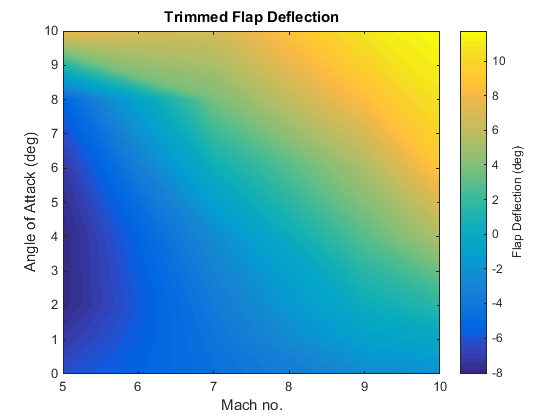
\includegraphics[width=0.99\linewidth]{figures/3_vehicle_design/FlapDeflectionENgineOn2}
	\caption{}
	\label{fig:FlapDeflectionENgineOn2}
\end{subfigure}
\begin{subfigure}{.5\textwidth}
	\centering
	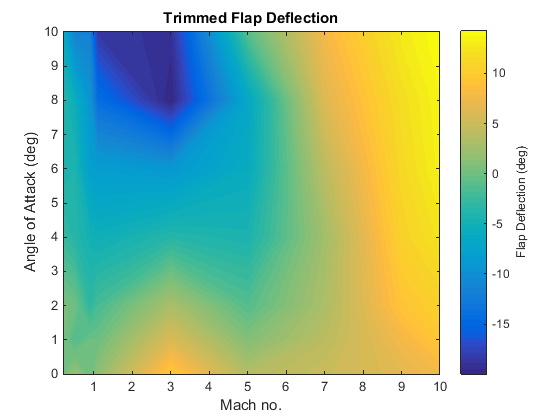
\includegraphics[width=0.99\linewidth]{figures/3_vehicle_design/FlapDeflection}
	\caption{}
	\label{fig:FlapDeflectionEngineOff}
\end{subfigure}
\label{fig:FlapDeflection}
\caption{Flap deflection required for trim of the SPARTAN. Negative up.}
\end{figure}

\subsection{Engine-On Plume Model}\label{sec:engine-on}

The operation of the scramjet engines changes the aerodynamic characteristics of the SPARTAN significantly. 
The plumes of the scramjet engines exit the nozzle of the SPARTAN, and are further expanded onto the boat tail on the rear of the SPARTAN fuselage. This expansion causes significant force on the boat tail of the SPARTAN, generating additional lift, thrust and moment forces. The plumes of the SPARTAN have been simulated using CART3D, using SurfBC boundary conditions which produce inflow and outflow conditions at the inlet and exit of the scramjet engines\cite{Pandya2004}. 

\begin{figure}
	\centering
	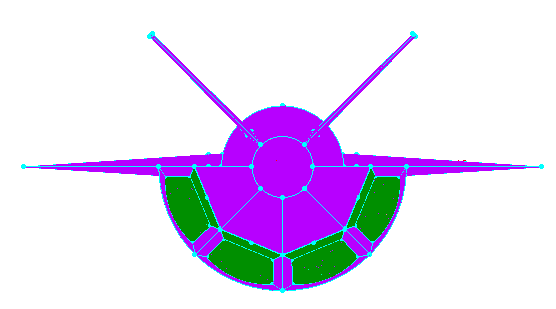
\includegraphics[width=0.7\linewidth]{figures/3_vehicle_design/Pointwise-EngineBC}
	\caption{Pointwise view of the SPARTAN showing engine outlet boundaries.}
	\label{fig:Pointwise-EngineBC}
\end{figure}

The CRESTM10 database has been used to calculate the engine conditions at the exit of the scramjet engines, and this has been set as the outflow condition. These conditions are normalised for CART3D as follows CITATIONXX:

\begin{equation}
P_e^* = P_e/(\gamma_0 P_0)
\end{equation}

\begin{equation}
\rho_e^* = \rho_e/\rho_0
\end{equation}

\begin{equation}
M_e^* = \sqrt{\gamma_e/\gamma_0 (M_e \sqrt{ P_e^*/\rho_e^*})^2}
\end{equation}
This includes a correction on the Mach number to account for $\gamma_e$ variation, which is not possible to include directly in CART3D\cite{Mehta2016}.

\begin{figure}
	\centering
	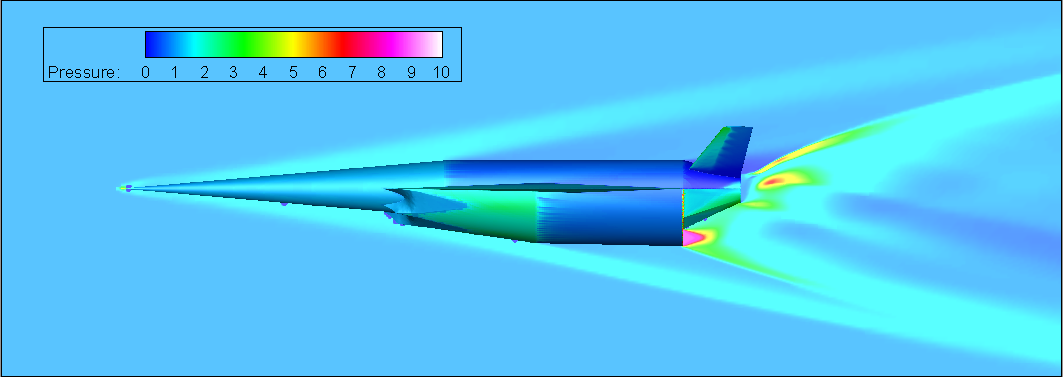
\includegraphics[width=0.9\linewidth]{figures/3_vehicle_design/EngineOn-M7AoA024km}
	\caption{}
	\label{fig:EngineOn-M7AoA624km}
\end{figure}


\section{First Stage Rocket}
The first stage rocket-powered vehicle is based on the first stage of the SpaceX Falcon-1e. The Falcon-1e has been chosen due to its appropriate scale, and the proven flightworthiness of the Falcon-1.

\begin{itemize}
	\item detailed design
	\item First Stage aerodynamic coefficients calculated in CART3D
	\item details of CAD, pointwise mesh, and CART3D gridding settings
\end{itemize}


  \subsubsection{Aerodynamics Including First Stage}

  
  The aerodynamics of the SPARTAN and first stage rocket have been calculated using CART3D. For the purposes of these simulations, a connecting cowl has been modelled between the first stage rocket and the SPARTAN, to improve aerodynamics. The first stage aerodynamics have been modelled between angles of attack of 0$^\circ$ to -5$^\circ$, as the first stage will be flying at negative angle of attack to induce faster pitch-over. Mach numbers from 0.2 to 5.1 (second stage separation velocity) have been simulated. Figure \ref{fig:CARTcontour} shows an example CART3D simulation case, at Mach 2, -1$^\circ$ angle of attack. Figure \ref{fig:FirstStageAero} shows the lift and drag coefficients of the first stage, as well as the lift-over-drag, across the simulated Mach Numbers and angles of attack. 
  
  
  
  \begin{figure}
  	\centering
  	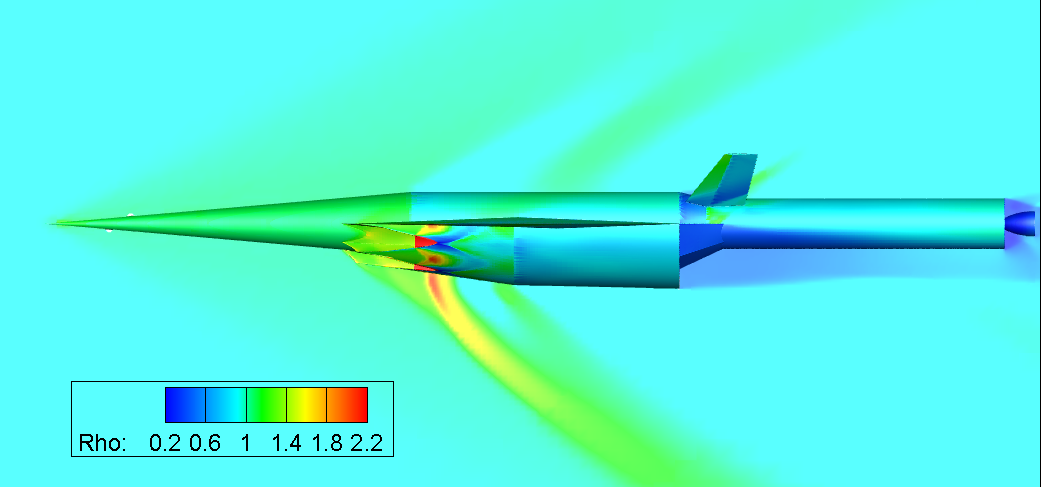
\includegraphics[width=0.7\linewidth]{figures/3_vehicle_design/CARTcontour}
  	\caption{CART3D result for the SPARTAN and first stage vehicles at Mach 2, -1$^\circ$ angle of attack.}
  	\label{fig:CARTcontour}
  \end{figure}

\begin{figure}
	\begin{subfigure}{.5\textwidth}
		\centering
		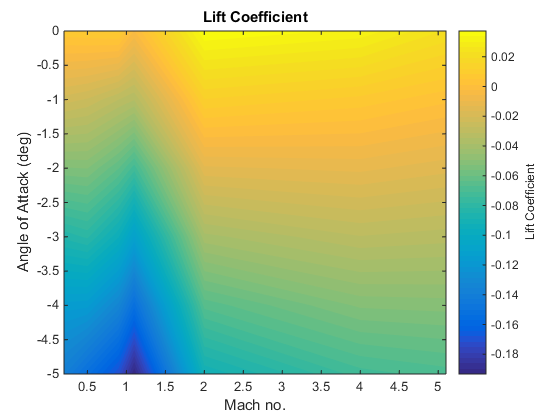
\includegraphics[width=0.99\linewidth]{figures/3_vehicle_design/FirstStageCl}
		\caption{Coefficient of lift.}
		\label{fig:Cl-FirstStage}
	\end{subfigure}
	\begin{subfigure}{.5\textwidth}
		\centering
		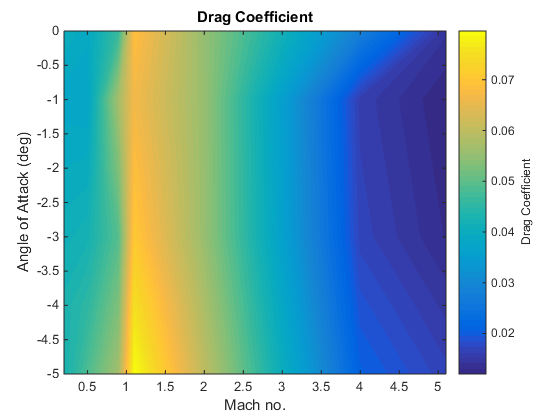
\includegraphics[width=0.99\linewidth]{figures/3_vehicle_design/FirstStageCd}
		\caption{Coefficient of drag.}
		\label{fig:Cd-FirstStage}
	\end{subfigure}
	\begin{subfigure}{.5\textwidth}
		\centering
		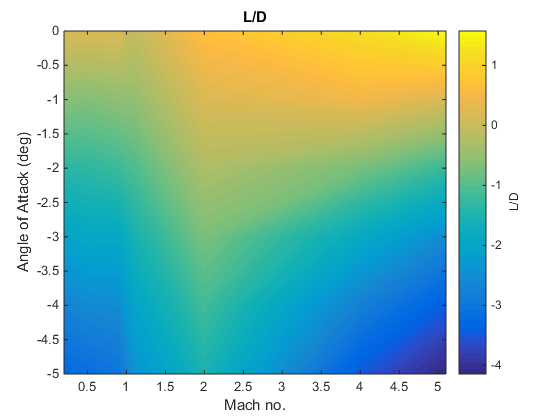
\includegraphics[width=0.99\linewidth]{figures/3_vehicle_design/FirstStageLD}
		\caption{L/D.}
		\label{fig:LD-EFirstStage}
	\end{subfigure}
	\caption{Aerodynamic characteristics of the SPARTAN including the first stage rocket.}
	\label{fig:FirstStageAero}
\end{figure}


	

	\section{Third Stage Rocket - Baseline}
	
	\begin{figure}
\centering
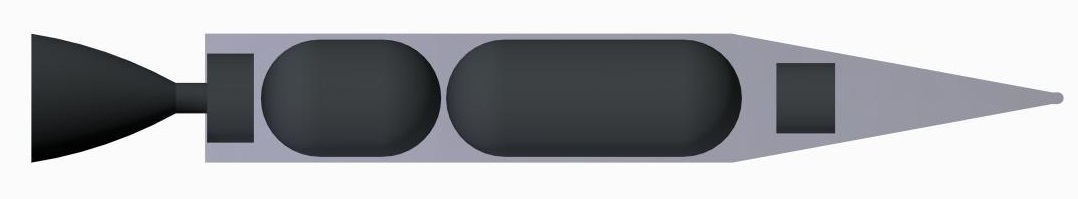
\includegraphics[width=0.7\linewidth]{figures/3_vehicle_design/3rdStage}
\caption{}
\label{fig:3rdStage}
\end{figure}
	
	In this study the third stage rocket has been designed to accommodate a SpaceX Kestrel engine. In previous studies, the third stage was designed to be powered by a Pratt \& Whitney RL-10-3A pump-fed engine, weighing 52kg. The Kestrel has been used over the RL-10-3A for its cost effectiveness. As a pressure-fed engine, the Kestrel trades off specific impulse for weight and cost savings when compared to the RL-10-3A. As the only expendable portion of the system; the cost of the third stage is one of the main drivers of overall system cost. Reducing the cost of the third stage allows the cost of launch to be directly reduced. 
	
	The third stage rocket is released at the end of the scramjet accelerator burn, and lifts the payload out of the atmosphere and into the desired orbit. The third stage weighs a total of 3300kg. This was chosen as a design weight, to fit the fuel necessary to achieve orbit with an acceptable payload while also allowing for ample payload volume. The third stage has a structural mass fraction of 0.09, similar to the Falcon 1 second stage \cite{Vehicle2008}. This gives a total structural mass of 285.7kg. 
	
	

	
The kestrel engine has been modified to have 50\% increased propellant mass flow rate, giving a mass flow rate of 14.8kg/s. The nozzle of the Kestrel engine has been kept at 1.1m diameter. This increase in mass flow results in a 2\% loss of efficiency from the nozzle\cite{RPE}, due to the thrust coefficient decreasing as shown in Figure \ref{fig:ThrustCoefficient-Arat}. The modified specific impulse of the engine is 310.7s.

\textcolor{red}{Arat initial is 60 (reference, measured I think), after thrust increase Arat is 40}

The third stage has a total length of 9m, with a 3m long nose, 4.5m long centrebody and 1.5m long engine.
	
	The centre of gravity is determined using CREO, and is at XXm from the nose. It is assumed that the mass of the structure of the rocket (excluding fuel tanks, heat shielding, engine and payload) is distributed homogeneously, for simplicity.
	
	
	\begin{figure}
\centering
\includegraphics[width=0.7\linewidth]{"figures/3_vehicle_design/Thrust Coefficient - Arat"}
\caption{\cite{RPE}}
\label{fig:ThrustCoefficient-Arat}
\end{figure}



\subsection{Heat Shield Sizing}
\textcolor{red}{present more of the logic which led to this heat shield design}

The third stage rocket is separated from the SPARTAN at a high dynamic pressure, after which it spends a considerable amount of time accelerating in-atmosphere before reaching exoatmospheric conditions. This release into a high dynamic pressure environment creates a large amount of heating, which must be mitigated by heat shielding. 
The third stage is protected while in-atmosphere by a heat shield, weighing 130.9kg. This heat shield is constructed from a phenolic cork cylinder, a reinforced carbon-carbon nose cone, and a tungsten nose tip. 
The tungsten nose is 50mm diameter, at the end of a 50mm cylinder. The density of tungsten is $\rho_{Tungsten} = 19.25$  g/cm$^3$, giving a total mass for the nose of m = 12.6kg.
The carbon-carbon shell has a density of $\rho_{CC} = 1800$  kg/m$^3$. The carbon-carbon shell has a thickness of 10mm. The mass of the carbon-carbon is 89.3kg. 
The cork cylinder has a density of $\rho_{Cork} = 320$  kg/m$^3$, a thickness of 5mm and a total mass of 23.7kg. 
The total mass of the heat shield is 125.6kg.

\textcolor{red}{put info in table}
		
		\subsection{Fuel Tank Sizing}
		The fuel tanks have been sized assuming 100kg of payload-to-orbit. Note that the method of calculating final payload-to-orbit relies on using left over 'fuel mass' as effective payload mass. Realistically this would cause the fuel tanks to be resized slightly. For the purposes of this study the fuel tanks have been assumed to be of constant size for simplicity. Currently this is a reasonable assumption as the internals of the rocket are very simplified. The structural mass is held constant at 9\%. The third stage carries a total propellant mass of 2736.7kg. Table XX breaks shows the component break-down of the LOX oxidiser and RP1 fuel.  
		
\begin{tabular}{|c|c|c|}
	\hline  & \textbf{LOX} & \textbf{RP1} \\ 
	\hline Ratio & 2.56 & 1 \\ 
	\hline Density & 1141kg/m3 & 813kg/m3 \cite{Magee}\\ 
	\hline Volume & 1.7248m3 & 0.9455m3 \\ 
	\hline Mass & 1968.0 kg & 768.7 kg \\ 
	\hline 
\end{tabular} 
		
		\textcolor{red}{it needs to be clearer here that the fuel tanks have been approximately sized, and that some fuel / payload is interchangeable}
		
		
		
		
		\subsection{Aerodynamics}
		
		The third stage aerodynamics have been calculated using Missile DATCOM [REFXX], a preliminary design tool for estimating the aerodynamic characteristics of missile and rocket vehicles. Missile DATCOM utilises empirical methods, along with various estimation techniques, to compute the aerodynamics of missile-like vehicles across the subsonic, supersonic and hypersonic regimes.  The code used to compute the aerodynamics of the third stage rocket is detailed in Appendix XX.  
		
		
		\begin{figure}
			\begin{subfigure}{.5\textwidth}
				\centering
				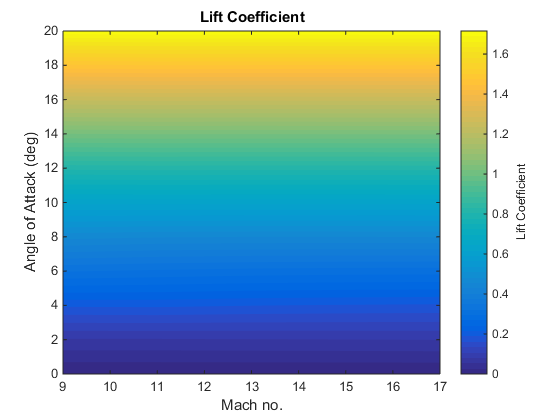
\includegraphics[width=0.99\linewidth]{figures/3_vehicle_design/ThirdStageCl}
				\caption{Coefficient of lift.}
				\label{fig:Cl-ThirdStage}
			\end{subfigure}
			\begin{subfigure}{.5\textwidth}
				\centering
				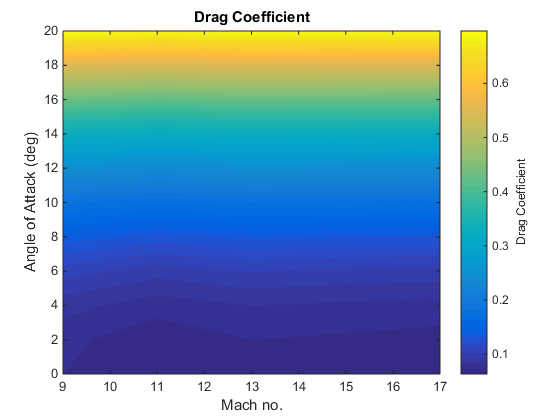
\includegraphics[width=0.99\linewidth]{figures/3_vehicle_design/ThirdStageCd}
				\caption{Coefficient of drag.}
				\label{fig:Cd-ThirdStage}
			\end{subfigure}
			\begin{subfigure}{.5\textwidth}
				\centering
				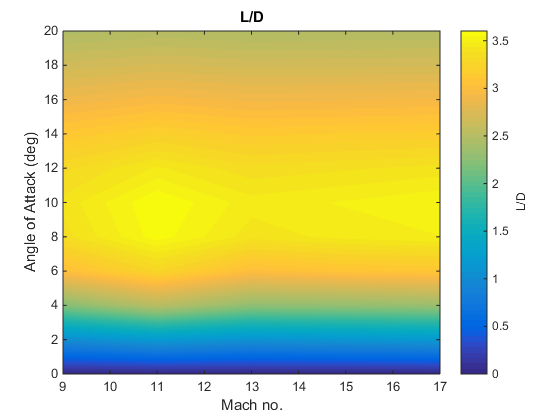
\includegraphics[width=0.99\linewidth]{figures/3_vehicle_design/ThirdStageLD}
				\caption{L/D.}
				\label{fig:LD-ThirdStage}
			\end{subfigure}
			\caption{Aerodynamic characteristics of the baseline third stage rocket, for a reference area of 0.95m$^2$.}
			\label{fig:ThirdStageAero}
		\end{figure}
		
		
		
		\subsection{Thrust Vectoring}
		
		The third stage rocket is trimmed during the in-atmosphere portion of its ascent trajectory via thrust vectoring. The centre of pressure is calculated using missile DATCOM. The thrust vector is set so that the moment generated by the engine matches the lift force acting at the centre of pressure. The maximum thrust vector limit has been set to 8$^\circ$. As no data on the maximum thrust vectoring capabilities of the kestrel engine was able to be found, this was set to the maximum gimbal range of the Aestus pressure-fed engine and OMS, similar pressure fed engines. 
		
		\textcolor{red}{add a diagram}
		

		